% exercise sheet with header on every page for math or close subjects
\documentclass[12pt]{article}
\usepackage[utf8]{inputenc} 
\usepackage{latexsym} 
\usepackage{multicol}
\usepackage{fancyhdr}
\usepackage{amsfonts} 
\usepackage{amsmath}
\usepackage{amssymb}
\usepackage{enumerate}
\usepackage{listings}
\usepackage{graphicx}
\usepackage{hyperref}

% Shortcuts for bb, frak and cal letters
\newcommand{\E}{\mathbb{E}}
\newcommand{\V}{\mathbb{V}}
\renewcommand{\P}{\mathbb{P}}
\newcommand{\N}{\mathbb{N}}
\newcommand{\R}{\mathbb{R}}
\newcommand{\C}{\mathbb{C}}
\newcommand{\Z}{\mathbb{Z}}
\newcommand{\Pfrak}{\mathfrak{P}}
\newcommand{\Pfrac}{\mathfrak{P}}
\newcommand{\Bfrac}{\mathfrak{P}}
\newcommand{\Bfrak}{\mathfrak{B}}
\newcommand{\Fcal}{\mathcal{F}}
\newcommand{\Ycal}{\mathcal{Y}}
\newcommand{\Bcal}{\mathcal{B}}
\newcommand{\Acal}{\mathcal{A}}

% formating
\topmargin -1.5cm 
\textheight 24cm
\textwidth 16.0 cm 
\oddsidemargin -0.1cm

% Fancy Header on every Page
\pagestyle{fancy}
\lhead{\textbf{Pattern and Speech Recognition}}
\rhead{Daniel Schäfer (2549458)\\ Christian Bohnenberger (2548364) \\ Dominik Weber (2548553)}
\renewcommand{\headrulewidth}{1.2pt}

\setlength{\headheight}{45pt} 

\begin{document}
\pagenumbering{gobble}

% TODO set the number of the exercise sheet here!
\setcounter{section}{7}
\setcounter{subsection}{0}

\subsection{ }

\begin{enumerate}[a)]
	\item see files in source folder
	
	\item 
		\begin{tabular}{|c|c|}
			\hline
 		 	Optimizer & Accuracy \\
 		 	\hline
 		 	gradient descent & 0.8883 \\
 		 	\hline
 		 	gradient descent with momentum(0.5) & 0.9109 \\
 		 	\hline
 		 	Adagrad (accumulaotr value=0.1) & 0.6359\\
 		 	\hline
 		 	RMSProp (decay=0.9, momentum=0) & 0.9299 \\
 		 	\hline
 		\end{tabular}
 		
 	\item 
 	Gradient descent is computed to the complete data set (or a batch if tensorflow implements gradient batch size) and only in the end one update is done. Here there is only one learning rate and each parameter is updated with this learning rate, hence we change every parameter with the same rate.\\
 	In Adagard a different way to update the weights/parameters is used. Here the learning rate is adapted to the parameters. In particular larger updates are performed for infrequent parameters, whereas smaller updates are performed for frequent parameters since you have more data to update the weights more slowly and carefully. This performs normally very well and outperforms gradient descent, however there are also cases in which the learning rate becomes very small such that the parameters are no longer updated. This could happen here. Furthermore the number of epochs is very small in comparison and the parameters are updated with smaller weights in comparison to the gradient descent approach. That's also a reason why gradient could be better in this example.\\
\end{enumerate}


\subsection{ }

\begin{enumerate}[a)]
    \item 
        see file \verb!gradient_descent.py!

    \item
        see file \verb!gradient_descent_momentum.py!

    \item
        in yellow you can see gradient descent with momentum and in red you can see ``normal'' gradient descent.\\
        \begin{center}
            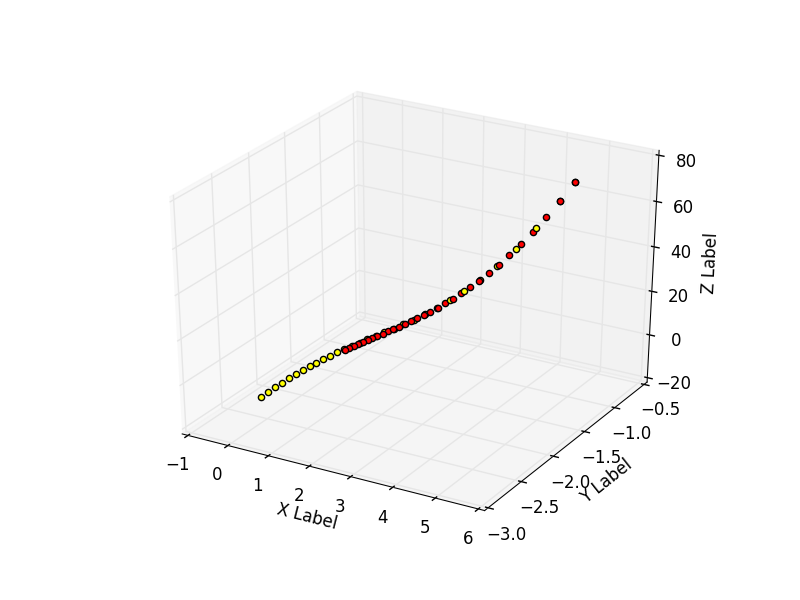
\includegraphics[scale = 0.8]{pictures/figure_1}\\
        \end{center}

    \item
        as you can clearly see in the plot above gradient descent with momentum is progressing a lot faster than without (with the values we used).\\

        \textbf{with momentum after 30 iterations:}
        \begin{verbatim}
        X = 0.23111880569092993
        Y = -2.6012090540073087
        f(x,y) = -6.60604083562
        \end{verbatim}

        \textbf{without momentum after 30 iterations:}
        \begin{verbatim}
        X = 0.831146841312047
        Y = -1.7758446902974057
        f(x,y) = -1.08120914859
        \end{verbatim}

    \item
        % TODO
        see file \verb!newtons_method.py!\\
        I added newtons method performance with 5 iterations in the plot in blue:\\
        \begin{center}
            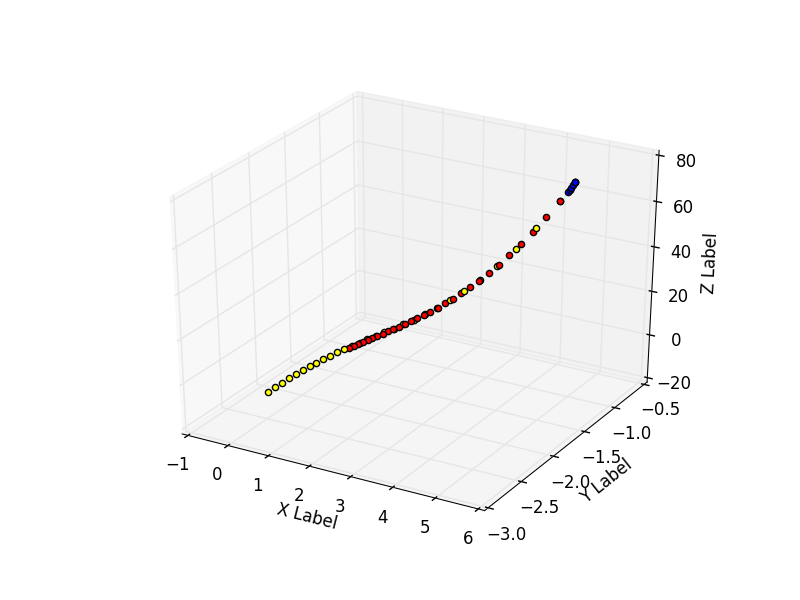
\includegraphics[scale = 0.8]{pictures/figure_2}\\
        \end{center}

        as one can clearly see it is performing so much worse than both gradient descent with and without momentum, that it is clearly not suited for this task!


\end{enumerate}


\subsection{ }

\begin{enumerate}[a)]
    \item 
        Gradient descent needs to much iterations for this flat function and can not reach the minima in 300 iterations.

\end{enumerate}

\end{document}
